\section{Finite effects - data space estimators}
\label{sec:fin-effs}

\subsection{New data, new processes}
\label{sec:new-dat}

We first show the bias and variance of each fit to see how stable the variance
is across fits compared to the bias for new data, new processes. The variance is
expected to be independent of the level 1 shift and so we assume any variation
is due to finite number of replicas.

\begin{figure}[!b]
    \centering
    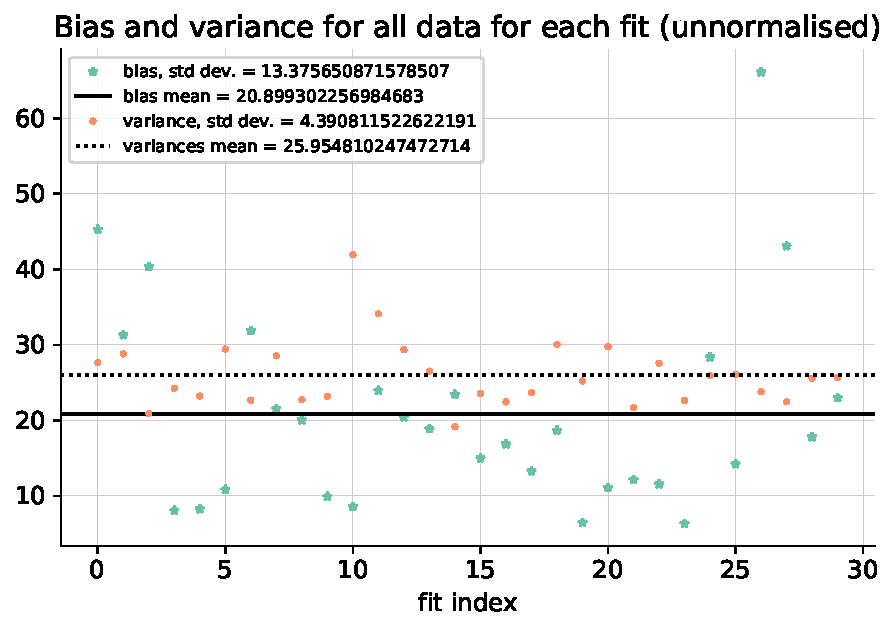
\includegraphics[width=0.6 \textwidth]{fullout_bias_variance_fits.pdf}
    \caption{Bias and variance for each fit for all new data, new processes. Each
    fit has 40 replicas. The variance is still fluctuating a fair amount and
    so results may be subject to finite statistics effects.}
    \label{fig:outnewfitbiasvar}
\end{figure}

\FloatBarrier

Next we use bootstrapping to try and gauge the dependence of the error on the
number of fits and replicas. Using the full set of fits and replicas as the
sample we draw a random subset of $\nfits$ fits and for each fit a random subset
of $\nreps$ replicas. We then calculate the estimators discussed in previous
sections for the resample of fits and replicas. For each value of $\nfits$ and
$\nreps$ we perform 100 bootstraps and then take the mean and standard deviation
of the estimator across bootstrap samples. Finally we vary $\nfits$ and $\nreps$
and tabulate the results in order to get an idea of the dependence of the error
on increasing the number of fits or replicas without having the redo any fits.

First we show the mean of bias/variance across bootstrap samples, varying
$\nfits$ and $\nreps$.
%
\begin{table}[h!]
    \label{tab:fullout_finite_effects_ratio_mean}
    \begin{center}
    \begin{tabular}{lrrrrr}
        \toprule
        {} & \multicolumn{5}{c}{$\nfits$} \\
        {} &   10 &   15 &   20 &   25 &   30 \\
        $\nreps$ &      &      &      &      &      \\
        \midrule
        25            & 0.90 & 0.88 & 0.88 & 0.88 & 0.90 \\
        30            & 0.87 & 0.90 & 0.85 & 0.87 & 0.88 \\
        35            & 0.88 & 0.85 & 0.88 & 0.86 & 0.87 \\
        40            & 0.88 & 0.84 & 0.85 & 0.84 & 0.85 \\
        \bottomrule
        \end{tabular}
\end{center}
    \caption{Bias/variance ratio as the number of fits and the number of replicas are varied.}
\end{table}

\FloatBarrier

Now the standard deviation across bootstrap samples of bias/variance, varying
$\nfits$ and $\nreps$
%
\begin{table}[h!]
    \label{tab:fullout_finite_effects_ratio_error}
    \begin{center}
    \begin{tabular}{lrrrrr}
        \toprule
        {} & \multicolumn{5}{c}{$\nfits$} \\
        {} &   10 &   15 &   20 &   25 &   30 \\
        $\nreps$ &      &      &      &      &      \\
        \midrule
        25            & 0.19 & 0.16 & 0.13 & 0.12 & 0.11 \\
        30            & 0.19 & 0.19 & 0.14 & 0.11 & 0.11 \\
        35            & 0.20 & 0.14 & 0.15 & 0.12 & 0.11 \\
        40            & 0.21 & 0.15 & 0.13 & 0.11 & 0.11 \\
        \bottomrule
        \end{tabular}
\end{center}
    \caption{Standard deviation of the bias/variance ratio as the number of fits and the number of replicas are varied.}
\end{table}

\FloatBarrier

Now we show the corresponding tables for the $\xi_{1\sigma}$ estimator. First
the mean across bootstrap samples

\begin{table}[h!]
    \label{tab:fullout_finite_effects_xi_mean}
    \begin{center}
    \begin{tabular}{lrrrrr}
        \toprule
        {} & \multicolumn{5}{c}{$\nfits$} \\
        {} &   10 &   15 &   20 &   25 &   30 \\
        $\nreps$ &      &      &      &      &      \\
        \midrule
        25            & 0.66 & 0.66 & 0.66 & 0.66 & 0.65 \\
        30            & 0.67 & 0.66 & 0.67 & 0.67 & 0.66 \\
        35            & 0.67 & 0.67 & 0.67 & 0.67 & 0.67 \\
        40            & 0.67 & 0.68 & 0.67 & 0.68 & 0.67 \\
        \bottomrule
        \end{tabular}
\end{center}
    \caption{Mean value of $\xi_{1\sigma}$ over bootstrap samples as the number of fits and the number of replicas are varied.}
\end{table}

\FloatBarrier

Now the standard deviation across bootstrap samples

\begin{table}[h!]
    \label{tab:fullout_finite_effects_xi_error}
    \begin{center}
    \begin{tabular}{lrrrrr}
    \toprule
    {} & \multicolumn{5}{c}{$\nfits$} \\
    {} &   10 &   15 &   20 &   25 &   30 \\
    $\nreps$ &      &      &      &      &      \\
    \midrule
    25            & 0.05 & 0.04 & 0.03 & 0.03 & 0.03 \\
    30            & 0.04 & 0.05 & 0.04 & 0.03 & 0.03 \\
    35            & 0.05 & 0.04 & 0.04 & 0.03 & 0.03 \\
    40            & 0.06 & 0.04 & 0.03 & 0.03 & 0.03 \\
    \bottomrule
    \end{tabular}
\end{center}
    \caption{Standard deviation of $\xi_{1\sigma}$ over bootstrap samples as the number of fits and the number of replicas are varied.}
\end{table}

\FloatBarrier

\subsection{New data, old processes}

We include the same results for new data, old processes. The results are very
consistent with those calculated with new data, new processes and so we might
want to just group all new data together.

\begin{table}[h!]
    \label{tab:partialout_finite_effects_ratio_mean}
    \begin{center}
    \begin{tabular}{lrrrrr}
        \toprule
        {} & \multicolumn{5}{c}{$\nfits$} \\
        {} &   10 &   15 &   20 &   25 &   30 \\
        $\nreps$ &      &      &      &      &      \\
        \midrule
        25            & 0.88 & 0.87 & 0.87 & 0.87 & 0.88 \\
        30            & 0.87 & 0.88 & 0.85 & 0.85 & 0.86 \\
        35            & 0.85 & 0.85 & 0.87 & 0.85 & 0.86 \\
        40            & 0.85 & 0.83 & 0.85 & 0.83 & 0.84 \\
        \bottomrule
        \end{tabular}
\end{center}
    \caption{Bias/variance ratio as the number of fits and the number of replicas are varied. }
\end{table}

\begin{table}[h!]
    \label{tab:partialout_finite_effects_ratio_error}
    \begin{center}
    \begin{tabular}{lrrrrr}
        \toprule
        {} & \multicolumn{5}{c}{$\nfits$} \\
        {} &   10 &   15 &   20 &   25 &   30 \\
        $\nreps$ &      &      &      &      &      \\
        \midrule
        25            & 0.14 & 0.11 & 0.09 & 0.09 & 0.08 \\
        30            & 0.15 & 0.13 & 0.08 & 0.07 & 0.07 \\
        35            & 0.14 & 0.11 & 0.11 & 0.09 & 0.08 \\
        40            & 0.14 & 0.09 & 0.09 & 0.08 & 0.08 \\
        \bottomrule
        \end{tabular}
\end{center}
    \caption{Standard deviation of the bias/variance ratio as the number of fits and the number of replicas are varied. }
\end{table}

\begin{table}[h!]
    \label{tab:partialout_finite_effects_xi_means}
    \begin{center}
    \begin{tabular}{lrrrrr}
        \toprule
        {} & \multicolumn{5}{c}{$\nfits$} \\
        {} &   10 &   15 &   20 &   25 &   30 \\
        $\nreps$ &      &      &      &      &      \\
        \midrule
        25            & 0.68 & 0.68 & 0.68 & 0.68 & 0.68 \\
        30            & 0.69 & 0.68 & 0.69 & 0.69 & 0.69 \\
        35            & 0.69 & 0.70 & 0.69 & 0.69 & 0.69 \\
        40            & 0.69 & 0.70 & 0.69 & 0.70 & 0.70 \\
        \bottomrule
        \end{tabular}
\end{center}
    \caption{Mean value of $\xi_{1\sigma}$ over bootstrap samples as the number of fits and the number of replicas are varied.}
\end{table}

\begin{table}[h!]
    \label{tab:partialout_finite_effects_xi_error}
    \begin{center}
    \begin{tabular}{lrrrrr}
        \toprule
        {} & \multicolumn{5}{c}{$\nfits$} \\
        {} &   10 &   15 &   20 &   25 &   30 \\
        $\nreps$ &      &      &      &      &      \\
        \midrule
        25            & 0.04 & 0.03 & 0.02 & 0.02 & 0.02 \\
        30            & 0.03 & 0.03 & 0.02 & 0.02 & 0.02 \\
        35            & 0.04 & 0.03 & 0.03 & 0.02 & 0.02 \\
        40            & 0.04 & 0.03 & 0.02 & 0.02 & 0.02 \\
        \bottomrule
        \end{tabular}
\end{center}
    \caption{Standard deviation of $\xi_{1\sigma}$ over bootstrap samples as the number of fits and the number of replicas are varied.}
\end{table}
